% capitulo5_ecc.tex
% Capítulo 5: Criptografía de curvas elípticas (ECC)
%
% Autor: Leon Elliott Fuller
% Fecha: Junio 2026

\chapter{Criptografía de curvas elípticas (ECC)}
\label{ch:ecc}

\section{Introducción y motivación}
\label{sec:ecc-intro}

Los investigadores llevaban años buscando funciones más seguras para criptografía y en 1985 se propuso por primera vez el uso de curvas elípticas como base del problema del logaritmo discreto en un grupo \cite{koblitz1987,miller1986}. Se cree que las curvas elípticas ofrecen un nivel de seguridad equivalente al de RSA pero con tamaños de clave mucho menores. Para ilustrar la diferencia en términos intuitivos, comparemos la energía necesaria para romper los diferentes sistemas con la cantidad de agua que esa energía podría hervir \cite{rickard-ecc,lenstra2001selecting}:

\begin{itemize}
    \item Romper una clave RSA de 228 bits requiere menos energía que la necesaria para hervir una cucharadita de agua.
    \item Romper una clave ECC de 228 bits equivaldría a la energía necesaria para hervir toda el agua de la Tierra.
    \item Para obtener el mismo nivel de seguridad con RSA haría falta una clave de unos 2\,380 bits, lo cual es muy ineficiente en entornos con recursos limitados.
\end{itemize}

En la figura \ref{fig:ecc-hierarchy} se muestra la jerarquía de la criptografía de las curvas elípticas, y cómo es necesario poder tener de base lo que hemos explicado en los capítulos anteriores.

\begin{figure}[htbp]
    \centering
    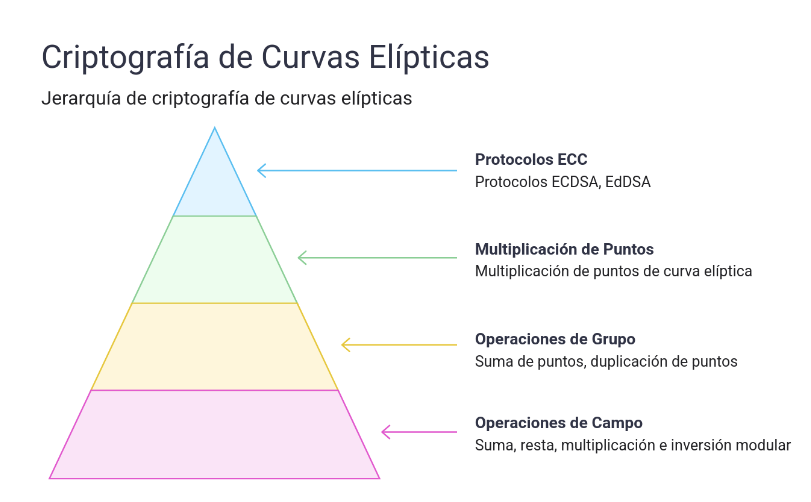
\includegraphics[width=0.7\textwidth]{imagenes/ECC_jerarquia.png}
    \caption{Jerarquía de la criptografía de Curvas Elípticas}
    \label{fig:ecc-hierarchy}
\end{figure}

\subsection{Historia}
\label{subsec:ecc-historia}

En 1997 Certicom lanzó el \emph{ECC Challenge} para evaluar la dificultad práctica del problema del logaritmo discreto en curvas elípticas \cite{gaudry2007breaking}. Pocos años después, en 1998, el comité ANSI X9 publicó la norma X9.62 definiendo el algoritmo de firma ECDSA, marcando el primer estándar formal para firmas basadas en curvas elípticas \cite{ansi-x962}. En el año 2000, el NIST incorporó curvas elípticas en el FIPS 186--2 (Digital Signature Standard), consolidando su uso en aplicaciones gubernamentales y financieras \cite{nist-fips186-2}.

En 2005 la NSA anunció la Suite B de algoritmos criptográficos, recomendando las curvas P-256, P-384 y P-521 para uso en comunicaciones seguras de nivel gubernamental \cite{rfc5430}. Con la adopción de TLS 1.2 y la publicación del RFC 8422 en 2018, las curvas secp256r1 (también conocida como prime256v1) y X25519 se convirtieron en cimientos de la seguridad de Internet, al ofrecer un excelente equilibrio entre rendimiento y seguridad \cite{rfc8422}. Más recientemente, TLS 1.3 (RFC 8446) ha consolidado aún más la posición de ECC al eliminar los \textit{cipher suites} basados exclusivamente en RSA para el intercambio de claves, favoreciendo ECDHE como mecanismo predeterminado \cite{rfc8446}.

En la actualidad, la criptografía de curvas elípticas es omnipresente y continúa evolucionando. Sin embargo, no ha estado exenta de desafíos: se han descubierto ataques teóricos contra curvas mal escogidas, y hubo polémicas como la del generador Dual-EC-DRBG (que involucraba curvas elípticas y una posible puerta trasera). Aun así, las curvas bien elegidas siguen considerándose seguras. Un punto a futuro es la computación cuántica: si llegaran a construirse ordenadores cuánticos a gran escala, los algoritmos de Shor podrían resolver el ECDLP eficientemente, rompiendo ECC al igual que RSA. Por ello, existe una carrera por desarrollar criptografía poscuántica. Pero hasta la fecha, ECC sigue siendo segura frente a ataques clásicos conocidos y representa uno de los pilares de la criptografía de clave pública contemporánea.


\subsection{Aplicaciones}
\label{subsec:ecc-aplicaciones}

Gracias a sus ventajas en seguridad y eficiencia, ECC se ha incorporado en numerosas aplicaciones modernas. A continuación destacamos algunas de las más relevantes:

\begin{description}
    \item[Blockchain y Criptomonedas:] Las curvas elípticas son la columna vertebral de la seguridad en blockchain. Por ejemplo, Bitcoin y Ethereum emplean la curva estándar secp256k1 junto con el algoritmo de firma digital ECDSA para gestionar las claves públicas y firmas de transacciones \cite{secp256k1-bitcoin}. Esto asegura que solo el poseedor de la clave privada correspondiente pueda autorizar movimientos de fondos.
    
    \item[Certificados Digitales y TLS/SSL:] ECC se utiliza en certificados X.509 para establecer identidades seguras en Internet. Muchas Autoridades de Certificación ofrecen certificados TLS basados en curvas elípticas (ECDSA o ECDH) como alternativa a los tradicionales RSA. La principal ventaja es que un certificado ECC puede lograr el mismo nivel de seguridad que RSA con claves de menor tamaño, acelerando el \textit{handshake} SSL/TLS y reduciendo la carga en servidores y clientes \cite{rfc4492,rfc5656}. Por ejemplo, un servidor web con un certificado ECDSA de 256 bits ofrece 128 bits de seguridad, equivalente a un RSA de 3072 bits \cite{hankerson2004guide}.
    
    \item[Sistemas de Mensajería y Cifrado de Extremo a Extremo (E2EE):] Protocolos modernos de mensajería segura, como Signal, WhatsApp o el protocolo de doble-ratchet de Olvid, utilizan intercambios de clave basados en curvas elípticas (por ejemplo, X25519, que es una curva elíptica de Montgomery). Estas aplicaciones aprovechan ECC para generar secretos compartidos de forma rápida y con alta seguridad en cada sesión de chat.
    
    \item[Firmas Digitales y Autenticación:] Más allá de los certificados TLS, ECC sustenta esquemas de firma digital ampliamente usados, como ECDSA y variantes más recientes como EdDSA (por ejemplo Ed25519). Estos se emplean en autenticación de documentos, en el DNIe de algunos países, en pasaportes biométricos, en tokens de hardware, etc. Por su eficiencia, ECC permite firmas y verificaciones rápidas incluso en dispositivos de recursos limitados (tarjetas inteligentes, dispositivos embebidos).
    
    \item[IoT y Dispositivos Embebidos:] En el Internet de las Cosas, donde muchos dispositivos tienen poca potencia de cómputo y batería limitada, ECC ha ganado protagonismo \cite{hodges2001ecc}. La posibilidad de usar claves más cortas y operaciones más eficientes hace viable implementar criptografía robusta en sensores, actuadores y \textit{wearables}.
\end{description}

Además, las propiedades algebraicas de las curvas han sido la base para esquemas avanzados como sistemas de emparejamientos (\textit{pairing-based cryptography}), identidades basadas en curva (IBE) y firmas Schnorr y EdDSA, ampliando enormemente el catálogo de construcciones criptográficas eficientes \cite{boneh2003ibe}.


% ============================================================================
\section{Fundamentos de ECC}
\label{sec:ecc-fundamentos}

\subsection{El problema del logaritmo discreto en curvas elípticas (ECDLP)}
\label{subsec:ecdlp}

La seguridad de todos los protocolos basados en curvas elípticas (ECDH, ECDSA, etc.) reposa sobre la dificultad computacional de un único problema: el \emph{problema del logaritmo discreto en curvas elípticas}.

\begin{definicion}[ECDLP]
\label{def:ecdlp}
Sea $E$ una curva elíptica definida sobre un cuerpo finito $\mathbb{F}_q$ y sea $P \in E(\mathbb{F}_q)$ un punto de orden primo $n$. Dado un punto $Q \in \langle P \rangle$ (el subgrupo cíclico generado por $P$), el \emph{problema del logaritmo discreto en curvas elípticas} (ECDLP) consiste en encontrar el entero $d$, con $0 \leq d \leq n-1$, tal que
\[
    Q = d \cdot P = \underbrace{P + P + \cdots + P}_{d \text{ veces}}.
\]
\end{definicion}

La operación $d \cdot P$ (multiplicación escalar) es eficiente: usando el algoritmo \textit{double-and-add} se calcula en $O(\log d)$ operaciones de grupo, es decir, $O(\log n)$ sumas y duplicaciones de puntos en la curva. Sin embargo, la operación inversa --dado $Q$ y $P$, encontrar $d$-- no admite ningún algoritmo eficiente conocido en el caso general.

\paragraph{Comparación con el DLP en $\mathbb{F}_p^*$.}
En el grupo multiplicativo $\mathbb{F}_p^*$, el problema del logaritmo discreto clásico (dado $g$ y $h = g^a \bmod p$, encontrar $a$) admite algoritmos sub-exponenciales como el \textit{index calculus}, cuya complejidad es $L_p\big[\tfrac{1}{3}, c\big] = e^{c(\ln p)^{1/3}(\ln \ln p)^{2/3}}$. Estos métodos explotan la estructura aritmética de $\mathbb{Z}/p\mathbb{Z}$ para ``factorizar'' elementos del grupo sobre una base de factores.

En curvas elípticas, no se conoce una versión efectiva del \textit{index calculus} para curvas generales sobre cuerpos primos: los mejores algoritmos conocidos son genéricos (es decir, se aplican a cualquier grupo cíclico) y no explotan ninguna estructura específica de la curva. Los más relevantes son:
\begin{itemize}
    \item \textbf{Baby-step/Giant-step} (Shanks): complejidad $O(\sqrt{n})$ en tiempo y espacio.
    \item \textbf{Rho de Pollard}: complejidad $O(\sqrt{n})$ en tiempo con espacio $O(1)$.
\end{itemize}

Ambos son de complejidad \emph{exponencial completa} respecto al tamaño de la entrada ($\log n$ bits). Es decir, para una curva de $k$ bits de seguridad, el mejor ataque conocido requiere $O(2^{k/2})$ operaciones. Esto implica que una curva de 256 bits ofrece aproximadamente 128 bits de seguridad, mientras que un RSA de 3072 bits es necesario para alcanzar ese mismo nivel \cite{hankerson2004guide,nist-sp800-57}.

\subsubsection{Baby-step / Giant-step (Shanks)}
\label{subsubsec:bsgs}
 
El algoritmo de Shanks \cite{hankerson2004guide} se basa en una idea elegante: descomponer el escalar desconocido $d$ en dos mitades y buscar una colisi\'on entre dos conjuntos precalculados.
 
\paragraph{Idea.}
Si escribimos $d = j \cdot m + i$ donde $m = \lceil \sqrt{n} \rceil$, con $0 \leq i < m$ y $0 \leq j < m$, entonces
\[
    Q = dP = (jm + i)P = jmP + iP
    \quad\Longrightarrow\quad
    Q - j(mP) = iP.
\]
El lado izquierdo depende solo de $j$ (``giant steps'') y el derecho solo de $i$ (``baby steps''). Si precalculamos todos los valores $iP$ y los almacenamos en una tabla hash, basta recorrer los giant steps hasta encontrar una coincidencia.
 
\begin{algorithm}[htbp]
\caption{Baby-step / Giant-step para el ECDLP}
\label{alg:bsgs}
\begin{algorithmic}[1]
\Require Puntos $P$, $Q \in E(\mathbb{F}_q)$ con $Q = dP$, orden $n = |P|$
\Ensure Entero $d$ tal que $Q = dP$
\State $m \leftarrow \lceil \sqrt{n} \rceil$
\State \Comment{\textbf{Baby steps}: precalcular $iP$ para $i = 0, 1, \ldots, m-1$}
\For{$i = 0$ \textbf{to} $m-1$}
    \State Almacenar $(iP, i)$ en tabla hash
\EndFor
\State \Comment{\textbf{Giant steps}: buscar colisi\'on}
\State $S \leftarrow Q$
\For{$j = 0$ \textbf{to} $m-1$}
    \If{$S$ est\'a en la tabla hash con valor $i$}
        \State \Return $d = jm + i \bmod n$
    \EndIf
    \State $S \leftarrow S - mP$ \Comment{Equivalente a $Q - (j+1)mP$}
\EndFor
\end{algorithmic}
\end{algorithm}
 
\paragraph{Complejidad.}
La fase de baby steps realiza $m$ multiplicaciones escalares y requiere $O(m)$ espacio para la tabla hash. La fase de giant steps realiza como m\'aximo $m$ sumas de puntos. El coste total es $O(m) = O(\sqrt{n})$ tanto en tiempo como en espacio. Para una curva de 256 bits, esto supone almacenar $\sim 2^{128}$ puntos, lo que es inviable con la tecnolog\'ia actual.
 
\begin{ejemplo}
\label{ej:bsgs}
Sea la curva $E: y^2 = x^3 + 2x + 3$ sobre $\mathbb{F}_{97}$, con generador $P = (0, 10)$ de orden $n = 50$ y objetivo $Q = (92, 81) = 16P$.
 
Calculamos $m = \lceil\sqrt{50}\rceil = 8$. Los baby steps son:
\begin{center}
\begin{small}
\begin{tabular}{cl}
$i$ & $iP$ \\
\hline
0 & $\mathcal{O}$ \\
1 & $(0, 10)$ \\
2 & $(65, 32)$ \\
3 & $(23, 24)$ \\
4 & $(52, 68)$ \\
5 & $(88, 56)$ \\
6 & $(95, 66)$ \\
7 & $(10, 76)$ \\
\end{tabular}
\end{small}
\end{center}
 
Para los giant steps, calculamos $8P = (84, 37)$ y recorremos $S_j = Q - j \cdot 8P$ para $j=0,1,2,\dots$ hasta encontrar una coincidencia con la tabla de baby steps. Concretamente, $S_0 = (92, 81)$ y $S_1 = (84, 37)$, ninguno de los cuales aparece en la tabla; en cambio, $S_2 = Q - 16P = \mathcal{O}$ coincide con la entrada $i = 0$. La colisi\'on se produce, por tanto, para $j = 2$, $i = 0$, dando $d = 2 \cdot 8 + 0 = 16$, como cab\'ia esperar de la construcci\'on $Q = 16P$.
\end{ejemplo}


\subsubsection{Método rho de Pollard}
\label{subsubsec:pollard-rho}

El rho de Pollard \cite{pollard1978monte} alcanza la misma complejidad temporal que BSGS ($O(\sqrt{n})$) pero con requerimiento de memoria constante $O(1)$, lo que lo convierte en el ataque más práctico contra el ECDLP \cite{hankerson2004guide}. Su nombre proviene de la forma de la letra griega $\rho$ que adopta la secuencia de puntos generada por el algoritmo.


\paragraph{La paradoja del cumpleaños.}
Antes de describir el algoritmo, conviene entender la observación probabilística que lo fundamenta. Consideremos la siguiente pregunta: ¿cuántas personas deben reunirse en una sala para que haya al menos un 50\,\% de probabilidad de que dos de ellas compartan cumpleaños?

Intuitivamente, como hay 365 días posibles, podríamos pensar que hacen falta muchas personas. Sin embargo, la respuesta es sorprendentemente baja: \textbf{basta con 23 personas}. Este resultado, conocido como la \emph{paradoja del cumpleaños}, se explica porque no buscamos que alguien comparta cumpleaños \emph{con una persona concreta}, sino que \emph{cualquier par} de personas coincida. Con $k$ personas, el número de pares posibles es $\binom{k}{2} = k(k-1)/2$, que crece cuadráticamente.

La probabilidad exacta de que al menos dos personas de un grupo de $k$ compartan cumpleaños (suponiendo $N = 365$ días equiprobables) se calcula como el complemento de que \emph{todos} tengan cumpleaños distintos:
\[
    P(k) = 1 - \prod_{i=0}^{k-1} \frac{N - i}{N}
         = 1 - \frac{N}{N} \cdot \frac{N-1}{N} \cdot \frac{N-2}{N} \cdots \frac{N-k+1}{N}.
\]

El cuadro \ref{tab:birthday} muestra los valores concretos.

\begin{table}[htbp]
\centering
\begin{tabular}{rc}
\hline
\textbf{Personas ($k$)} & \textbf{$P$(coincidencia)} \\
\hline
5   & 2.7\,\% \\
10  & 11.7\,\% \\
20  & 41.1\,\% \\
\textbf{23} & \textbf{50.7\,\%} \\
30  & 70.6\,\% \\
40  & 89.1\,\% \\
50  & 97.0\,\% \\
57  & 99.0\,\% \\
70  & 99.9\,\% \\
\hline
\end{tabular}
\caption{Probabilidad de que al menos dos personas compartan cumpleaños en un grupo de $k$ personas ($N = 365$ días).}
\label{tab:birthday}
\end{table}

El umbral del 50\,\% se alcanza con $k = 23 \approx \sqrt{\pi \cdot 365 / 2} \approx 1{,}25\sqrt{365}$. Esto no es casualidad: mediante una aproximación estándar ($\ln(1-x) \approx -x$ para $x$ pequeño), se demuestra que el número esperado de elementos que debemos elegir al azar de un conjunto de $N$ para encontrar una colisión es
\begin{equation}
\label{eq:birthday-bound}
    k \approx \sqrt{\frac{\pi N}{2}} \approx 1{,}25 \sqrt{N}.
\end{equation}

Nótese que este resultado es \emph{independiente} de qué elemento concreto se repita: solo depende del tamaño $N$ del conjunto.


\paragraph{De cumpleaños a curvas elípticas.}
El ataque rho de Pollard traslada esta observación al grupo de puntos de una curva elíptica. Si el generador $P$ tiene orden $n$, el subgrupo $\langle P \rangle$ contiene exactamente $n$ puntos distintos. Si generamos una secuencia de puntos pseudoaleatorios en este grupo, por la cota \eqref{eq:birthday-bound} esperamos encontrar una \emph{colisión} (dos índices $i \neq j$ con $x_i = x_j$) tras aproximadamente $\sqrt{\pi n/2} \approx 1{,}25\sqrt{n}$ pasos. Para una curva de 256 bits ($n \approx 2^{256}$), esto supone $\approx 2^{128}$ pasos, que es precisamente la seguridad que atribuimos a dicha curva. El cuadro \ref{tab:birthday-ecc} muestra esta correspondencia.

\begin{table}[htbp]
\centering
\begin{tabular}{ccc}
\hline
\textbf{Curva (bits)} & \textbf{Orden $n \approx$} & \textbf{Pasos esperados $\approx$} \\
\hline
160 & $2^{160}$ & $2^{80}$ \\
224 & $2^{224}$ & $2^{112}$ \\
256 & $2^{256}$ & $2^{128}$ \\
384 & $2^{384}$ & $2^{192}$ \\
521 & $2^{521}$ & $2^{260}$ \\
\hline
\end{tabular}
\caption{Número esperado de pasos del rho de Pollard según el tamaño de la curva. Los bits de seguridad son exactamente la mitad de los bits de la curva.}
\label{tab:birthday-ecc}
\end{table}

Pero la paradoja del cumpleaños, por sí sola, solo dice cuántos pasos necesitamos para una colisión. No dice cómo \emph{detectar} esa colisión eficientemente (sin almacenar los $\sqrt{n}$ puntos previos, lo cual requeriría tanto espacio como BSGS), ni cómo \emph{extraer} el logaritmo discreto de ella. Para esto se necesitan dos ingredientes: un \emph{paseo pseudoaleatorio con invariante} y la \emph{detección de ciclos de Floyd}.


\paragraph{El paseo pseudoaleatorio y el invariante.}
La idea clave de Pollard es construir la secuencia de puntos de forma \emph{determinista} pero que se \emph{comporte} como aleatoria, manteniendo en todo momento un invariante que permita recuperar $d$ al encontrar una colisión. Cada punto $R_i$ de la secuencia se escribe como $R_i = a_i P + b_i Q$ donde los coeficientes $a_i, b_i$ son conocidos.

El siguiente punto se calcula aplicando una regla que depende solo del punto actual, particionando el grupo en tres subconjuntos según la coordenada $x$ módulo 3:

\begin{center}
\begin{tabular}{clccc}
\hline
\textbf{Partición} & \textbf{Condición} & \textbf{Nuevo punto} & \textbf{Nuevo $a$} & \textbf{Nuevo $b$} \\
\hline
$S_1$ & $x_R \equiv 0 \pmod{3}$ & $R + Q$ & $a$ & $b + 1$ \\
$S_2$ & $x_R \equiv 1 \pmod{3}$ & $2R$ & $2a$ & $2b$ \\
$S_3$ & $x_R \equiv 2 \pmod{3}$ & $R + P$ & $a + 1$ & $b$ \\
\hline
\end{tabular}
\end{center}

Todos los cálculos de coeficientes se realizan módulo $n$. En los tres casos se preserva el invariante: si $R = aP + bQ$ antes del paso, el nuevo punto $R'$ también se expresa como $R' = a'P + b'Q$ con los coeficientes actualizados según la tabla.

\paragraph{¿Por qué estas tres operaciones?}
La elección no es arbitraria. Las tres reglas cumplen propiedades esenciales:

\begin{itemize}
    \item \textbf{Preservan el invariante.} Cada regla actualiza $(a, b)$ de forma que $R' = a'P + b'Q$ sigue siendo cierto. Esto es imprescindible para poder extraer $d$ al final.

    \item \textbf{La partición debe ser aproximadamente equilibrada.} Si los tres subconjuntos $S_1, S_2, S_3$ contienen aproximadamente $n/3$ puntos cada uno, el paseo se comporta como una función aleatoria sobre el grupo. Usar $x_R \bmod 3$ produce una distribución razonablemente uniforme para la mayoría de las curvas.

    \item \textbf{La duplicación ($S_2$) aporta ``mezcla''.} Si solo sumásemos $P$ o $Q$, el paseo sería demasiado regular (una progresión aritmética en los coeficientes). La duplicación introduce no linealidad en los coeficientes ($a \mapsto 2a$, $b \mapsto 2b$), haciendo que la secuencia ``salte'' por el grupo de forma menos predecible.
\end{itemize}

El punto inicial $R_0 = a_0 P + b_0 Q$ puede ser cualquier punto con coeficientes conocidos. La elección $a_0 = 1$, $b_0 = 0$ (es decir, $R_0 = P$) es simplemente la más sencilla.

\paragraph{Nota sobre cuerpos binarios.}
El algoritmo es \emph{idéntico} para curvas sobre $\mathbb{F}_{2^m}$: la partición se basa igualmente en la coordenada $x$ del punto, las tres reglas ($+Q$, $2R$, $+P$) utilizan la aritmética de grupo de la curva (que en $\mathbb{F}_{2^m}$ emplea las fórmulas de la sección \ref{subsec:ecc-campos-binarios}), y los coeficientes $(a, b)$ se actualizan módulo $n$ de la misma manera. La única diferencia es que las operaciones de cuerpo subyacentes (suma $=$ XOR, multiplicación de polinomios) son distintas, pero esto es transparente al nivel del algoritmo de Pollard.


\paragraph{\texorpdfstring{Estructura $\rho$.}{Estructura rho.}}
Dado que el grupo $\langle P \rangle$ es finito, la secuencia $x_0, x_1, x_2, \ldots$ necesariamente revisita algún punto, formando una cola de longitud $\lambda$ seguida de un ciclo de longitud $\mu$: se cumple $x_{\lambda + \mu} = x_\lambda$. Esta estructura se ilustra en la figura \ref{fig:rho-shape}.

\begin{figure}[htbp]
\centering
\begin{tikzpicture}[
    node distance=1.2cm,
    point/.style={circle, draw, fill=blue!20, minimum size=6mm, font=\small},
    cpoint/.style={circle, draw, fill=red!20, minimum size=6mm, font=\small},
    arrow/.style={->, >=stealth, thick}
]
% Cola (tail)
\node[point] (x0) {$x_0$};
\node[point, below of=x0] (x1) {$x_1$};
\node[point, below of=x1] (x2) {$x_\lambda$};

% Ciclo (cycle) - circular
\node[cpoint, below right=0.8cm and 1.5cm of x2] (x3) {$x_{\lambda\!+\!1}$};
\node[cpoint, right=1.4cm of x3] (x4) {};
\node[cpoint, above right=0.8cm and 0.6cm of x4] (x5) {};
\node[cpoint, above=1.2cm of x5] (x6) {};
\node[cpoint, above left=0.8cm and 0.6cm of x6] (x7) {};
\node[cpoint, left=1.4cm of x7] (x8) {$x_{\lambda\!+\!\mu}$};

% Arrows - tail
\draw[arrow, blue!60] (x0) -- (x1);
\draw[arrow, blue!60] (x1) -- node[left, font=\scriptsize, gray]{$\vdots$} (x2);
\draw[arrow, blue!60] (x2) -- (x3);

% Arrows - cycle
\draw[arrow, red!60] (x3) -- (x4);
\draw[arrow, red!60] (x4) -- (x5);
\draw[arrow, red!60] (x5) -- (x6);
\draw[arrow, red!60] (x6) -- (x7);
\draw[arrow, red!60] (x7) -- (x8);
\draw[arrow, red!60, bend left=20] (x8) to node[below, font=\scriptsize]{$= x_\lambda$} (x3);

% Braces
\draw[decorate, decoration={brace, amplitude=8pt, mirror}]
    ([xshift=-8mm]x0.north) -- ([xshift=-8mm]x2.south)
    node[midway, left=10pt, font=\small] {cola $\lambda$};
\node[right=2.5cm of x5, font=\small, text=red!70!black] {ciclo $\mu$};

\end{tikzpicture}
\caption{Estructura $\rho$ de la secuencia. Los primeros $\lambda$ puntos (azul) forman la cola. A partir de $x_\lambda$ la secuencia entra en un ciclo de longitud $\mu$ (rojo), cumpliéndose $x_{\lambda+\mu} = x_\lambda$.}
\label{fig:rho-shape}
\end{figure}


\paragraph{Detección de ciclos: tortuga y liebre de Floyd.}
Para detectar cuándo la secuencia se repite sin almacenar todos los puntos visitados, se emplean dos iteradores que recorren el \emph{mismo} paseo a velocidades distintas. Denotamos por $f$ la aplicación de un paso del paseo (elegir partición según $x_R \bmod 3$, actualizar punto y coeficientes). Entonces:
\begin{align}
    \text{Tortuga:} \quad t_i &= f(t_{i-1}) = x_i, \label{eq:tortuga}\\
    \text{Liebre:}  \quad \ell_i &= f(f(\ell_{i-1})) = x_{2i}. \label{eq:liebre}
\end{align}
La tortuga aplica $f$ una vez por iteración (avanza un paso en la secuencia) y la liebre aplica $f$ dos veces (avanza dos pasos). En cada iteración $i$ se comprueba si $t_i = \ell_i$. Puesto que la liebre recorre la secuencia al doble de velocidad, eventualmente ``alcanzará'' a la tortuga dentro del ciclo.

\paragraph{Extracción del logaritmo.}
Cuando se produce la colisión $t_i = \ell_i$, la tortuga y la liebre se encuentran en el mismo punto de la curva, pero llegaron por caminos distintos y por tanto tienen coeficientes potencialmente diferentes:
\[
    a_t P + b_t Q = a_\ell P + b_\ell Q.
\]
Sustituyendo $Q = dP$:
\[
    (a_t - a_\ell)P = (b_\ell - b_t) d P
    \quad\Longrightarrow\quad
    a_t - a_\ell \equiv (b_\ell - b_t) \cdot d \pmod{n}.
\]
Si $\gcd(b_\ell - b_t, n) = 1$ (lo cual ocurre con alta probabilidad cuando $n$ es primo), se despeja:
\begin{equation}
\label{eq:rho-recovery}
    d = (a_t - a_\ell) \cdot (b_\ell - b_t)^{-1} \bmod n.
\end{equation}


\paragraph{Pseudocódigo.}
El algoritmo \ref{alg:pollard-rho} detalla el procedimiento completo con la lógica de partición expandida, mostrando explícitamente cómo la tortuga aplica un paso y la liebre dos en cada iteración.

\begin{algorithm}[htbp]
\caption{Método $\rho$ de Pollard para el ECDLP}
\label{alg:pollard-rho}
\begin{algorithmic}[1]
\Require Puntos $P$, $Q \in E(\mathbb{F}_q)$ con $Q = dP$, orden primo $n = |P|$
\Ensure Entero $d$ tal que $Q = dP$
\State $t \leftarrow P$;\; $a_t \leftarrow 1$;\; $b_t \leftarrow 0$
    \Comment{Tortuga: $t = 1 \cdot P + 0 \cdot Q$}
\State $\ell \leftarrow P$;\; $a_\ell \leftarrow 1$;\; $b_\ell \leftarrow 0$
    \Comment{Liebre: igual inicio}
\Repeat
    \State \Comment{-- Tortuga: un paso --}
    \If{$x_t \equiv 0 \pmod{3}$}
        \State $t \leftarrow t + Q$;\; $b_t \leftarrow b_t + 1$
    \ElsIf{$x_t \equiv 1 \pmod{3}$}
        \State $t \leftarrow 2t$;\; $a_t \leftarrow 2a_t$;\; $b_t \leftarrow 2b_t$
    \Else
        \State $t \leftarrow t + P$;\; $a_t \leftarrow a_t + 1$
    \EndIf
    \State \Comment{-- Liebre: dos pasos --}
    \For{$j = 1$ \textbf{to} $2$}
        \If{$x_\ell \equiv 0 \pmod{3}$}
            \State $\ell \leftarrow \ell + Q$;\; $b_\ell \leftarrow b_\ell + 1$
        \ElsIf{$x_\ell \equiv 1 \pmod{3}$}
            \State $\ell \leftarrow 2\ell$;\; $a_\ell \leftarrow 2a_\ell$;\; $b_\ell \leftarrow 2b_\ell$
        \Else
            \State $\ell \leftarrow \ell + P$;\; $a_\ell \leftarrow a_\ell + 1$
        \EndIf
    \EndFor
    \State \Comment{Todos los coeficientes se reducen módulo $n$}
\Until{$t = \ell$}
\If{$b_\ell \equiv b_t \pmod{n}$}
    \State \Return \textbf{Fallo} (reintentar con otro punto inicial)
\Else
    \State \Return $d \leftarrow (a_t - a_\ell) \cdot (b_\ell - b_t)^{-1} \bmod n$
\EndIf
\end{algorithmic}
\end{algorithm}


\paragraph{Ejemplo numérico.}
Consideremos la curva $E\colon y^2 = x^3 + 2x + 1$ sobre $\mathbb{F}_{89}$, con punto generador $P = (1, 2)$ de orden primo $n = 47$. Sea $Q = (87, 73) = 15P$ el punto cuyo logaritmo discreto queremos encontrar.

Ambos iteradores parten de $t_0 = \ell_0 = P = (1,2)$ con coeficientes $(a, b) = (1, 0)$. En cada iteración, la tortuga aplica un paso del paseo y la liebre aplica dos. La siguiente tabla muestra el desarrollo completo:

\begin{center}
\begin{small}
\begin{tabular}{r|crrp{0.8cm}|crr|c}
\hline
 & \multicolumn{4}{c|}{\textbf{Tortuga} $t_i = x_i$} & \multicolumn{3}{c|}{\textbf{Liebre} $\ell_i = x_{2i}$} & \\
$i$ & Punto & $a_t$ & $b_t$ & Regla & Punto & $a_\ell$ & $b_\ell$ & $t_i\!=\!\ell_i$? \\
\hline
 0 & $(1, 2)$    &  1 &  0 & & $(1, 2)$    &  1 &  0 &  \\
 1 & $(83, 29)$  &  2 &  0 & $S_2$ & $(78, 28)$  &  3 &  0 & No \\
 2 & $(78, 28)$  &  3 &  0 & $S_3$ & $(10, 24)$  &  4 &  1 & No \\
 3 & $(38, 83)$  &  3 &  1 & $S_1$ & $(42, 83)$  &  9 &  2 & No \\
 4 & $(10, 24)$  &  4 &  1 & $S_3$ & $(3, 52)$   & 18 &  6 & No \\
 5 & $(80, 77)$  &  8 &  2 & $S_2$ & $(40, 1)$   & 19 &  7 & No \\
 6 & $(42, 83)$  &  9 &  2 & $S_3$ & $(18, 66)$  & 29 & 28 & No \\
 7 & $(4, 47)$   &  9 &  3 & $S_1$ & $(84, 69)$  & 11 & 11 & No \\
 8 & $(3, 52)$   & 18 &  6 & $S_2$ & $(38, 83)$  & 11 & 13 & No \\
 9 & $(38, 6)$   & 18 &  7 & $S_1$ & $(80, 77)$  & 24 & 26 & No \\
10 & $(40, 1)$   & 19 &  7 & $S_3$ & $(4, 47)$   & 25 & 27 & No \\
11 & $(13, 34)$  & 38 & 14 & $S_2$ & $(38, 6)$   &  3 &  8 & No \\
12 & $(18, 66)$  & 29 & 28 & $S_2$ & $(13, 34)$  &  8 & 16 & No \\
\textbf{13} & $\mathbf{(64, 48)}$ & \textbf{29} & \textbf{29} & $S_1$ & $\mathbf{(64, 48)}$ & \textbf{16} & \textbf{33} & \textbf{Sí} \\
\hline
\end{tabular}
\end{small}
\end{center}

Veamos en detalle cómo se obtiene la fila $i = 1$. La tortuga parte de $t_0 = (1, 2)$; como $x_{t_0} = 1 \equiv 1 \pmod{3}$, estamos en $S_2$ (duplicar), así que $t_1 = 2 \cdot (1, 2) = (83, 29)$ y los coeficientes se duplican: $(a_t, b_t) = (2, 0)$. La liebre parte del mismo punto pero aplica el paseo \emph{dos veces}: primero obtiene $(83, 29)$ (igual que la tortuga), y después, como $83 \equiv 2 \pmod{3}$ ($S_3$), suma $P$: $\ell_1 = (83, 29) + P = (78, 28)$ con $(a_\ell, b_\ell) = (2+1, 0) = (3, 0)$. La liebre ya está en $x_2$ de la secuencia mientras la tortuga está en $x_1$.

En el paso $i = 13$ se produce la colisión: $t_{13} = \ell_{13} = (64, 48)$. Los coeficientes son:
\[
    \text{Tortuga: } (64, 48) = 29P + 29Q, \qquad
    \text{Liebre: } (64, 48) = 16P + 33Q.
\]

Aplicando la ecuación \eqref{eq:rho-recovery}:
\begin{align*}
    a_t - a_\ell &= 29 - 16 = 13 \pmod{47}, \\
    b_\ell - b_t &= 33 - 29 = 4 \pmod{47}, \\
    4^{-1} &\equiv 12 \pmod{47} \quad (\text{pues } 4 \cdot 12 = 48 \equiv 1 \pmod{47}), \\
    d &= 13 \cdot 12 \bmod 47 = 156 \bmod 47 = \mathbf{15}.
\end{align*}
Verificamos: $15 \cdot P = 15 \cdot (1, 2) = (87, 73) = Q$. \qed

La secuencia pura generada por el paseo tiene cola $\lambda = 2$ (los puntos $x_0, x_1$ no se repiten) y ciclo $\mu = 13$ (desde $x_2$ hasta $x_{14}$, con $x_{15} = x_2$). La colisión de Floyd se produce en el paso 13 porque es el primer momento en que la tortuga (en $x_{13}$) y la liebre (en $x_{26}$, que por el ciclo coincide con $x_{13}$) se encuentran en el mismo punto. La figura \ref{fig:rho-visual} muestra la visualización de este proceso.

\begin{figure}[htbp]
    \centering
    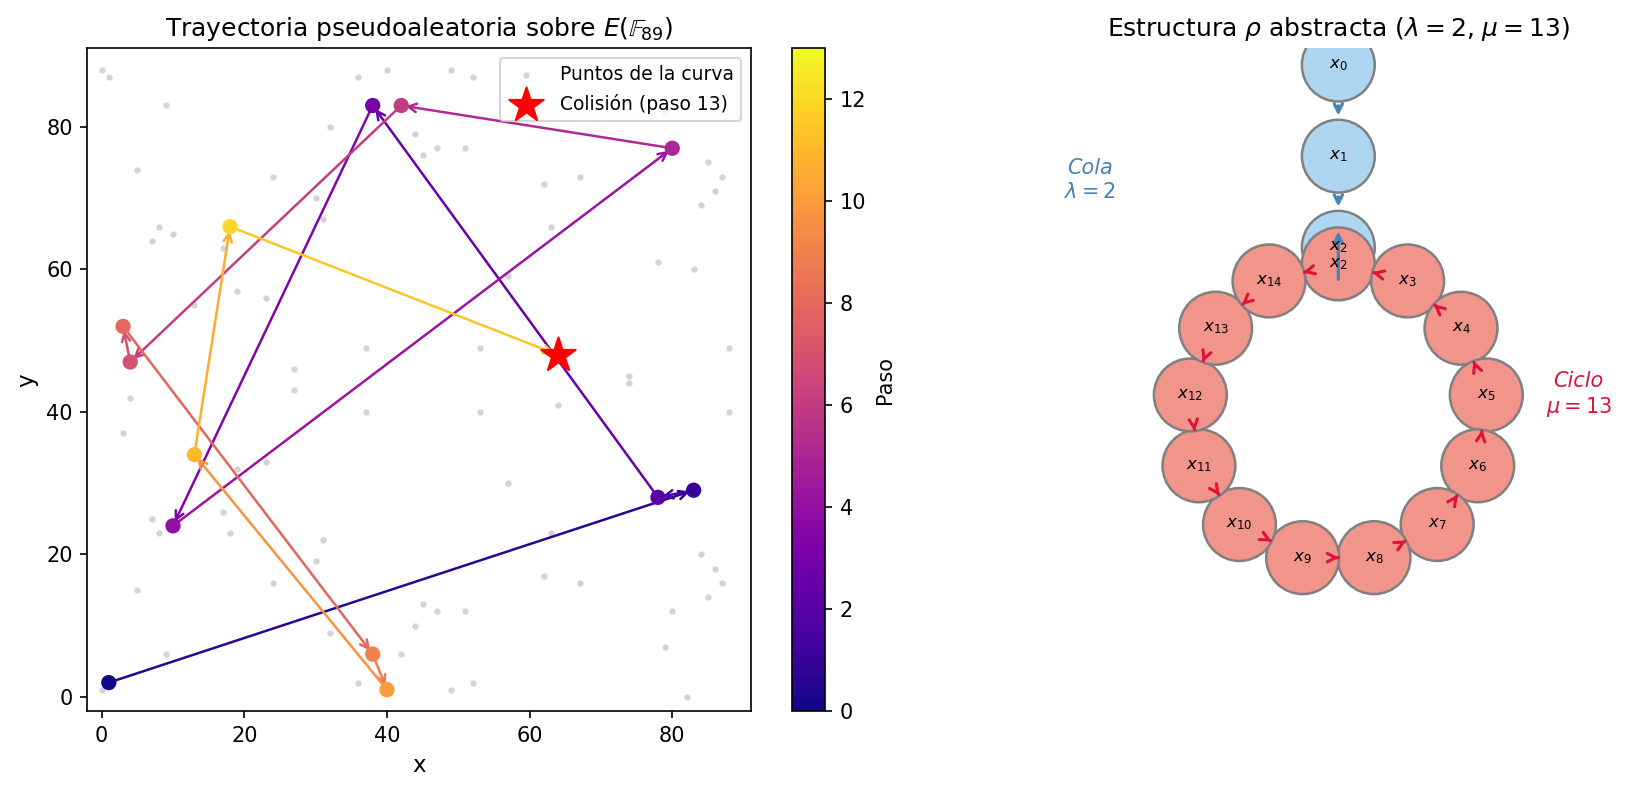
\includegraphics[width=\textwidth]{imagenes/attack_pollard_rho.png}
    \caption{Visualización del rho de Pollard sobre la curva $y^2 = x^3 + 2x + 1$ mod 89. Panel izquierdo: trayectoria pseudoaleatoria de la tortuga sobre la curva, coloreada por orden de aparición; la estrella marca la colisión en el paso 13. Panel derecho: estructura abstracta de $\rho$ mostrando la cola ($\lambda = 2$, azul) y el ciclo ($\mu = 13$, rojo).}
    \label{fig:rho-visual}
\end{figure}


\paragraph{Complejidad.}
El número esperado de iteraciones hasta la colisión es $O(\sqrt{n})$ por la paradoja del cumpleaños (cuadro \ref{tab:birthday-ecc}). Cada iteración consiste en una operación de grupo para la tortuga y dos para la liebre. Crucialmente, el método de Floyd solo almacena dos puntos y sus coeficientes en cada momento: espacio $O(1)$. Esto supone una ventaja decisiva frente a BSGS, que necesita $O(\sqrt{n})$ espacio para su tabla hash.

Para una curva de 256 bits con $n \approx 2^{256}$, el ataque requiere $\approx 2^{128}$ operaciones, fuera del alcance computacional actual. El récord práctico fue la resolución de la curva ECC2K-130 (130 bits sobre cuerpo binario) en 2009, tras un esfuerzo de cálculo distribuido masivo \cite{gaudry2007breaking}.

\begin{observacion}
    El rho de Pollard es un \emph{algoritmo genérico}: no explota ninguna propiedad específica de las curvas elípticas, solo la estructura de grupo finito cíclico. Funciona de forma idéntica sobre cuerpos primos $\mathbb{F}_p$ y cuerpos binarios $\mathbb{F}_{2^m}$, ya que solo depende de la operación de grupo (suma de puntos), no de la aritmética del cuerpo subyacente. Esta genericidad es, paradójicamente, la razón por la que ECC es segura: a diferencia de los ataques \textit{index calculus} contra el DLP en $\mathbb{F}_p^*$ (que explotan la estructura aritmética del cuerpo), no se conoce forma de acelerar el ataque en curvas elípticas más allá de $O(\sqrt{n})$.
\end{observacion}

\subsection{Comparativa de tamaños de clave}
\label{subsec:ecc-comparativa-claves}

La ausencia de ataques sub-exponenciales en curvas elípticas tiene una consecuencia práctica directa: ECC necesita claves drásticamente más pequeñas que RSA para ofrecer el mismo nivel de seguridad. El cuadro \ref{tab:ecc-rsa-equiv} resume las equivalencias según el NIST SP 800-57 \cite{nist-sp800-57}.

\begin{table}[htbp]
\centering
\begin{tabular}{cccc}
\hline
\textbf{Seguridad (bits)} & \textbf{RSA (bits)} & \textbf{ECC (bits)} & \textbf{Relación RSA/ECC} \\
\hline
80  & 1024  & 160 & 6.4:1 \\
112 & 2048  & 224 & 9.1:1 \\
128 & 3072  & 256 & 12:1 \\
192 & 7680  & 384 & 20:1 \\
256 & 15360 & 521 & 29.5:1 \\
\hline
\end{tabular}
\caption{Equivalencia de niveles de seguridad entre RSA y ECC según NIST SP 800-57.}
\label{tab:ecc-rsa-equiv}
\end{table}

La relación RSA/ECC \emph{crece} a medida que aumenta el nivel de seguridad deseado. Esto se debe a que la complejidad del mejor ataque a RSA (criba del cuerpo numérico general, sub-exponencial) escala peor que la del mejor ataque a ECC (Pollard rho, exponencial). En la práctica, esto se traduce en:

\begin{itemize}
    \item Menor consumo de ancho de banda (certificados TLS más pequeños).
    \item Generación de claves más rápida (generar un escalar aleatorio de 256 bits es trivial comparado con encontrar dos primos de 1536 bits).
    \item Operaciones criptográficas más eficientes, especialmente relevante en dispositivos con recursos limitados (IoT, tarjetas inteligentes).
\end{itemize}


\subsection{Parámetros del dominio de una curva elíptica}
\label{subsec:ecc-parametros-dominio}

Para instanciar un criptosistema basado en curvas elípticas, todas las partes involucradas deben acordar un conjunto de \emph{parámetros del dominio}. En el caso de curvas sobre cuerpos primos $\mathbb{F}_p$, estos parámetros se definen como la séxtupla
\[
    T = (p,\; a,\; b,\; G,\; n,\; h),
\]
donde:
\begin{itemize}
    \item $p$ es un primo que define el cuerpo finito $\mathbb{F}_p$.
    \item $a, b \in \mathbb{F}_p$ son los coeficientes de la ecuación de Weierstrass $y^2 = x^3 + ax + b$.
    \item $G = (G_x, G_y) \in E(\mathbb{F}_p)$ es el \emph{punto generador} (o \emph{base point}).
    \item $n$ es el \emph{orden} de $G$, es decir, el menor entero positivo tal que $n \cdot G = \mathcal{O}$.
    \item $h = \#E(\mathbb{F}_p) / n$ es el \emph{cofactor}.
\end{itemize}

Para que los parámetros proporcionen seguridad criptográfica adecuada, deben satisfacer varios requisitos \cite{sec2-v2,hankerson2004guide}:

\begin{enumerate}
    \item $n$ debe ser primo (o al menos tener un factor primo muy grande). Esto garantiza que el subgrupo $\langle G \rangle$ sea cíclico de orden primo, eliminando ataques basados en la estructura de subgrupos (Pohlig--Hellman).
    \item El cofactor $h$ debe ser pequeño (idealmente $h = 1$). Si $h > 1$, existen puntos de orden bajo que podrían utilizarse en ataques de curva inválida (\textit{invalid curve attacks}).
    \item La curva no debe ser \emph{anómala}: $\#E(\mathbb{F}_p) \neq p$. Las curvas anómalas son vulnerables al ataque de Smart--Semaev--Satoh, que resuelve el ECDLP en tiempo lineal mediante un levantamiento $p$-ádico \cite{smart1999anomalous}.
    \item La curva no debe tener \emph{grado de inmersión} bajo: $p^k \not\equiv 1 \pmod{n}$ para $k$ pequeño (típicamente $k > 20$). Las curvas con grado de inmersión bajo son vulnerables a ataques de emparejamiento de Weil y Tate (ataque MOV/Frey--Rück), que reducen el ECDLP a un DLP en $\mathbb{F}_{p^k}^*$ \cite{menezes1993reducing}.
    \item El discriminante de la curva debe ser no nulo: $\Delta = -16(4a^3 + 27b^2) \neq 0$.
\end{enumerate}

\subsection{Generación y verificación de parámetros de dominio}
\label{subsec:ecc-gen-verificacion-params}

Los parámetros del dominio $T = (p, a, b, G, n, h)$ pueden obtenerse de dos formas: adoptando una curva estandarizada (como hacemos en nuestra implementación) o generando parámetros nuevos siguiendo un procedimiento riguroso. En ambos casos, es fundamental verificar que los parámetros satisfacen los requisitos de seguridad. A continuación describimos ambos procesos, siguiendo la exposición de Hankerson, Menezes y Vanstone \cite{hankerson2004guide}.

\subsubsection{\texorpdfstring{Generación de parámetros sobre $\mathbb{F}_p$}{Generacion de parametros sobre Fp}}
\label{subsubsec:gen-params-fp}

El proceso de generación de una curva elíptica segura sobre un cuerpo primo $\mathbb{F}_p$ consta de los siguientes pasos:

\begin{enumerate}
    \item \textbf{Selección del primo $p$.} Se elige un primo $p$ de tamaño adecuado al nivel de seguridad deseado (por ejemplo, 256 bits para 128 bits de seguridad). Para eficiencia, se prefieren primos con estructura especial que facilite la reducción modular, como los \emph{primos pseudo-Mersenne} usados por el NIST (e.g., $p_{256} = 2^{256} - 2^{224} + 2^{192} + 2^{96} - 1$).
    
    \item \textbf{Selección de los coeficientes $a$ y $b$.} Se eligen $a, b \in \mathbb{F}_p$ tales que el discriminante $\Delta = -16(4a^3 + 27b^2) \neq 0$. Para curvas verificablemente aleatorias (\textit{verifiably random}), los coeficientes se derivan de una semilla $s$ mediante una función hash: $b = H(s)$, publicando $s$ para que cualquiera pueda verificar que no se seleccionó maliciosamente.
    
    \item \textbf{Conteo de puntos.} Se calcula $N = \#E(\mathbb{F}_p)$ mediante el algoritmo de Schoof--Elkies--Atkin (SEA), cuya complejidad es polinómica en $\log p$ \cite{schoof1985elliptic}. Este es el paso computacionalmente más costoso del proceso de generación.
    
    \item \textbf{Verificación del orden.} Se comprueba que $N$ tiene un factor primo grande $n$ con cofactor pequeño: $N = hn$ con $h \leq 4$ (idealmente $h = 1$).
    
    \item \textbf{Verificaciones de seguridad adicionales:}
    \begin{itemize}
        \item La curva no es anómala: $N \neq p$.
        \item El grado de inmersión es alto: $p^k \not\equiv 1 \pmod{n}$ para $1 \leq k \leq 20$.
        \item (Opcional) El endomorfismo de la curva no tiene estructura explotable.
    \end{itemize}
    
    \item \textbf{Selección del generador $G$.} Se elige un punto aleatorio $P \in E(\mathbb{F}_p)$ y se calcula $G = hP$. Se verifica que $G \neq \mathcal{O}$, lo que garantiza que $G$ tiene orden $n$.
\end{enumerate}

Si alguna verificación falla, se repite el proceso con nuevos coeficientes.

\subsubsection{\texorpdfstring{Generación de parámetros sobre $\mathbb{F}_{2^m}$}{Generacion de parametros sobre F2m}}
\label{subsubsec:gen-params-f2m}

El proceso es análogo pero con diferencias propias de la característica 2:

\begin{enumerate}
    \item \textbf{Selección del grado $m$.} Se elige $m$ primo o con propiedades adecuadas. Se prefieren valores para los que existan polinomios irreducibles trinomiales o pentanomiales, que permiten reducción eficiente.
    
    \item \textbf{Selección del polinomio irreducible $f(x)$.} Se elige un polinomio irreducible de grado $m$ sobre $\mathbb{F}_2$, preferentemente trinomial ($x^m + x^k + 1$) por eficiencia.
    
    \item \textbf{Selección de los coeficientes.} Para la ecuación $y^2 + xy = x^3 + ax^2 + b$, se requiere $b \neq 0$ (condición de no singularidad). Las curvas de Koblitz fijan $a \in \{0, 1\}$ para obtener optimizaciones con el endomorfismo de Frobenius.
    
    \item \textbf{Conteo de puntos y verificaciones.} Igual que en el caso primo, usando algoritmos adaptados a la característica 2.
\end{enumerate}


\subsubsection{Verificación de parámetros de dominio}
\label{subsubsec:verificacion-params}

La verificación de parámetros de dominio es esencial cuando se reciben de un tercero o se adoptan de un estándar. El algoritmo \ref{alg:verify-params} resume las comprobaciones necesarias para curvas sobre $\mathbb{F}_p$ \cite{hankerson2004guide,sec1-v2}.

\begin{algorithm}[htbp]
\caption{Verificación de parámetros de dominio $(p, a, b, G, n, h)$}
\label{alg:verify-params}
\begin{algorithmic}[1]
\Require Parámetros del dominio $T = (p, a, b, G, n, h)$
\Ensure \textbf{Válido} o \textbf{Inválido}
\State Verificar que $p$ es primo y $p > 3$.
\State Verificar que $a, b \in [0, p-1]$ y $4a^3 + 27b^2 \not\equiv 0 \pmod{p}$.
\State Verificar que $G \neq \mathcal{O}$ y que $G$ está en la curva: $G_y^2 \equiv G_x^3 + aG_x + b \pmod{p}$.
\State Verificar que $n$ es primo.
\State Verificar que $n \cdot G = \mathcal{O}$. \Comment{$G$ tiene orden $n$}
\State Verificar que $h = \lfloor (\sqrt{p} + 1)^2 / n \rfloor$. \Comment{Cofactor correcto}
\State Verificar que $hn \neq p$ (no anómala).
\State Verificar que $p^k \not\equiv 1 \pmod{n}$ para $1 \leq k \leq 20$. \Comment{Grado de inmersión alto}
\State \Return \textbf{Válido}
\end{algorithmic}
\end{algorithm}

\paragraph{Nuestra implementación.}
En nuestro proyecto utilizamos exclusivamente curvas estandarizadas por el NIST \cite{nist-fips186-4} y SECG \cite{sec2-v2}, cuyos parámetros han sido auditados y verificados por la comunidad criptográfica. Nuestra función \texttt{CurveParams::validate()} implementa las comprobaciones 1--3 y 6 (parcialmente) del algoritmo \ref{alg:verify-params}: discriminante no nulo, punto generador en la curva, y valores positivos de $n$ y $h$. Las verificaciones 4, 5, 7 y 8 no se implementan por ser redundantes con los parámetros de estándares publicados, pero se describen como requisitos teóricos. En un sistema que aceptase curvas arbitrarias definidas por el usuario, su implementación sería imprescindible.

De forma análoga, \texttt{BinaryCurveParams::validate()} comprueba que el grado del polinomio irreducible coincide con $m$, que $b \neq 0$ (discriminante no nulo en característica 2), y que $n$ y $h$ son positivos.

La validación de claves públicas se realiza en el constructor de \texttt{ECPoint}, que verifica automáticamente $y^2 = x^3 + ax + b \pmod{p}$ al crear cualquier punto, lanzando una excepción si el punto no pertenece a la curva. Para las curvas con cofactor $h = 1$ (NIST P-256, P-384, secp256k1), esta verificación es suficiente, ya que todo punto no trivial de la curva tiene orden $n$. Para curvas con $h > 1$ (como las binarias sect233k1 con $h = 4$), sería necesario verificar adicionalmente que $n \cdot Q = \mathcal{O}$ para garantizar la pertenencia al subgrupo correcto, lo que se documenta como limitación del prototipo.


% ============================================================================
\section{Generación de claves}
\label{sec:ecc-keygen}

La generación de un par de claves ECC es conceptualmente sencilla: la clave privada es un escalar aleatorio y la clave pública es el punto resultante de multiplicar el generador por dicho escalar.

\begin{definicion}[Par de claves ECC]
\label{def:ecc-keypair}
Dados los parámetros del dominio $T = (p, a, b, G, n, h)$, un par de claves ECC $(d, Q)$ se genera como sigue:
\begin{enumerate}
    \item Seleccionar un entero aleatorio $d$ uniformemente distribuido en el rango $[1, n-1]$.
    \item Calcular el punto $Q = d \cdot G$.
\end{enumerate}
La clave privada es $d$ y la clave pública es $Q$.
\end{definicion}

Dado que $n$ es primo y $d \in [1, n-1]$, el punto $Q$ es un elemento no trivial de $\langle G \rangle$. Conocer $Q$ y $G$ no permite recuperar $d$ eficientemente, por la dificultad del ECDLP (definición \ref{def:ecdlp}).

\paragraph{Requisitos del generador de números aleatorios.}
La seguridad del par de claves depende críticamente de la calidad del generador de números aleatorios (RNG) utilizado para seleccionar $d$. Si el RNG es predecible, sesgado o tiene baja entropía, un atacante podría reducir drásticamente el espacio de búsqueda de $d$. En nuestra implementación, empleamos el RNG de NTL inicializado con una semilla de alta entropía, cuya calidad estadística fue validada en la fase 2 del proyecto mediante tests de uniformidad, autocorrelación y rachas (véase el capítulo de implementación).

\paragraph{Validación de la clave pública.}
Al recibir una clave pública $Q$ de un tercero, es imprescindible verificar que:
\begin{enumerate}
    \item $Q \neq \mathcal{O}$ (no es el punto en el infinito).
    \item $Q$ pertenece a la curva: $Q_y^2 \equiv Q_x^3 + aQ_x + b \pmod{p}$.
    \item $Q$ pertenece al subgrupo correcto: $n \cdot Q = \mathcal{O}$.
\end{enumerate}
La tercera comprobación es especialmente importante cuando $h > 1$, para prevenir ataques de contribución de subgrupo pequeño \cite{hankerson2004guide}.


% ============================================================================
\section{Intercambio de claves: ECDH}
\label{sec:ecdh}

El protocolo de Diffie--Hellman sobre curvas elípticas (ECDH) es la adaptación directa del intercambio de claves Diffie--Hellman clásico (sección \ref{sec:diffie_hellman}) al grupo de puntos de una curva elíptica. Su seguridad se fundamenta en el \emph{problema de Diffie--Hellman computacional en curvas elípticas} (ECDHP): dados $P$, $aP$ y $bP$, calcular $abP$.

\subsection{Protocolo básico}
\label{subsec:ecdh-protocolo}

Sean Alice y Bob dos entidades que desean establecer un secreto compartido. Ambos acuerdan previamente los parámetros del dominio $T = (p, a, b, G, n, h)$. El protocolo se desarrolla de la siguiente manera:

\begin{enumerate}
    \item \textbf{Generación de claves.} Alice genera su par de claves $(d_A, Q_A)$ con $Q_A = d_A \cdot G$, y Bob genera $(d_B, Q_B)$ con $Q_B = d_B \cdot G$.
    \item \textbf{Intercambio público.} Alice envía $Q_A$ a Bob, y Bob envía $Q_B$ a Alice. Un intruso observa $Q_A$ y $Q_B$ pero no conoce $d_A$ ni $d_B$.
    \item \textbf{Cálculo del secreto compartido.} Alice calcula
    \[
        S = d_A \cdot Q_B = d_A \cdot (d_B \cdot G) = d_A d_B \cdot G,
    \]
    y Bob calcula
    \[
        S = d_B \cdot Q_A = d_B \cdot (d_A \cdot G) = d_B d_A \cdot G.
    \]
    Ambos obtienen el mismo punto $S$ gracias a la asociatividad y conmutatividad de la multiplicación escalar.
    \item \textbf{Derivación de clave.} La coordenada $x$ del punto $S$ (o una función de derivación de clave aplicada sobre ella) se utiliza como clave simétrica de sesión.
\end{enumerate}

\begin{figure}[htbp]
\centering
\begin{tikzpicture}[
    font=\small,
    actor/.style={draw, rounded corners, fill=blue!12, minimum width=2.2cm,
                  minimum height=0.8cm, align=center, font=\bfseries},
    life/.style={draw=gray!55, dashed, thick},
    msg/.style={-{Latex[length=2.5mm]}, thick, blue!50!black},
    note/.style={draw, rounded corners, align=left, font=\footnotesize,
                 inner sep=4pt, text width=4.4cm},
    noteA/.style={note, fill=teal!8,   draw=teal!60},
    noteB/.style={note, fill=orange!8, draw=orange!60},
    mlbl/.style={font=\scriptsize\sffamily, fill=white, inner sep=1.5pt}
]
    % Actores y lineas de vida
    \node[actor] (A) at (0,0) {Alice};
    \node[actor] (B) at (7,0) {Bob};
    \draw[life] (A.south) -- (0,-9.7);
    \draw[life] (B.south) -- (7,-9.7);

    % Intercambio publico de las claves de largo plazo
    \draw[msg] (0,-4.3) -- node[mlbl,above]{$Q_A$} (7,-4.3);
    \draw[msg] (7,-5.1) -- node[mlbl,above]{$Q_B$} (0,-5.1);

    % Generacion de claves (en paralelo)
    \node[noteA, align=center] (aKey) at (0,-2.1)
        {\textbf{1. Generación de claves}\\
        $d_A \gets [1,n-1]$\\
        $Q_A = d_A \cdot G$};
        
    \node[noteB, align=center] (bKey) at (7,-2.1)
        {\textbf{1. Generación de claves}\\
        $d_B \gets [1,n-1]$\\
        $Q_B = d_B \cdot G$};

    % Calculo independiente del mismo secreto compartido
    \node[noteA] (aSec) at (0,-7.0)
        {\textbf{2. Secreto compartido}\\
         $S = d_A \cdot Q_B = d_A d_B\,G$\\
         Clave: $k = x_S \bmod 2^{b}$};
    \node[noteB] (bSec) at (7,-7.0)
        {\textbf{2. Secreto compartido}\\
         $S = d_B \cdot Q_A = d_A d_B\,G$\\
         Clave: $k = x_S \bmod 2^{b}$};

    % Nota central
    \node[draw, rounded corners, fill=gray!8, align=center, font=\footnotesize,
          text width=8.6cm, inner sep=4pt] at (3.5,-9.1)
        {Ambos obtienen el mismo punto $S$. En el prototipo la clave es la
         coordenada $x_S$ truncada a $b$ bits, sin aplicar una KDF.};
\end{tikzpicture}
\caption{Diagrama de secuencia del intercambio de claves ECDH tal como se implementa en el prototipo. Alice y Bob generan sus pares de claves de largo plazo, intercambian las claves públicas $Q_A$ y $Q_B$ y calculan de forma independiente el mismo punto secreto $S = d_A d_B\,G$. La clave de sesión se obtiene directamente de la coordenada $x_S$ truncada al tamaño deseado de $b$ bits, sin función de derivación (véase la sección~\ref{subsec:ecdh-kdf}).}
\label{fig:ecdh-secuencia}
\end{figure}

\begin{table}[htbp]
\centering
\begin{tabular}{ll}
\hline
\textbf{Fase} & \textbf{Operación} \\
\hline
Acuerdo público & Parámetros $T = (p, a, b, G, n, h)$ \\
Generación de claves & Alice: $d_A \gets [1, n-1],\; Q_A = d_A \cdot G$ \\
                      & Bob: \quad $d_B \gets [1, n-1],\; Q_B = d_B \cdot G$ \\
Intercambio público & Alice $\to$ Bob: $Q_A$ \quad Bob $\to$ Alice: $Q_B$ \\
Secreto compartido & Alice: $S = d_A \cdot Q_B$ \quad Bob: $S = d_B \cdot Q_A$ \\
\hline
\end{tabular}
\caption{Resumen del intercambio de claves ECDH.}
\label{tab:ecdh-summary}
\end{table}


\begin{ejemplo}
\label{ej:ecdh-numerico}
Consideremos la curva $E: y^2 = x^3 + 2x + 3$ sobre $\mathbb{F}_{97}$ con punto generador $G = (3, 6)$ de orden $n = 5$.

Alice elige $d_A = 3$ y calcula $Q_A = 3 \cdot G = (80, 10)$. Bob elige $d_B = 4$ y calcula $Q_B = 4 \cdot G = (80, 87)$.

Alice calcula $S = 3 \cdot Q_B = 3 \cdot (80, 87) = (3, 91)$ y Bob calcula $S = 4 \cdot Q_A = 4 \cdot (80, 10) = (3, 91)$. Ambos obtienen el punto $S = (3, 91)$ como secreto compartido, y podrían usar $x_S = 3$ como semilla para derivar una clave simétrica.
\end{ejemplo}


\subsection{Derivación de claves}
\label{subsec:ecdh-kdf}

En la práctica, la coordenada $x$ del punto compartido $S$ no se utiliza directamente como clave simétrica, sino que se pasa por una \emph{función de derivación de clave} (KDF, \textit{Key Derivation Function}). Las razones son:

\begin{itemize}
    \item La coordenada $x$ puede tener bits con distribución no uniforme (por ejemplo, los bits más significativos pueden estar correlacionados con la estructura del cuerpo).
    \item Se necesita adaptar la longitud del secreto al tamaño de la clave simétrica deseada (128, 192 o 256 bits para AES).
    \item Un KDF aporta una capa adicional de seguridad: aunque se descubriese alguna debilidad parcial en la coordenada $x$, la clave derivada permanece segura si el KDF es robusto.
\end{itemize}

En estándares como NIST SP 800-56A \cite{nist-sp800-56a} se especifican KDFs basados en funciones hash, como HKDF (RFC 5869). En nuestra implementación educativa utilizamos directamente la coordenada $x$ truncada al número de bits deseados, anotando esta simplificación como limitación del prototipo.


\subsection{Variantes y extensiones}
\label{subsec:ecdh-variantes}

Existen varias variantes del intercambio ECDH que mejoran distintos aspectos del protocolo:

\begin{description}
    \item[ECIES (\textit{Elliptic Curve Integrated Encryption Scheme}):] Combina ECDH con un cifrado simétrico y un MAC en un esquema de cifrado de clave pública completo. Definido en IEEE P1363a e ISO 18033-2, es el análogo de ElGamal sobre curvas elípticas. La Figura~\ref{fig:ecies-simplificado} muestra una versión \emph{simplificada} de este esquema realizada con las primitivas del prototipo (ECDH y derivación por truncamiento, sin KDF ni MAC).
    
    \item[X25519:] Diseñada por Bernstein \cite{bernstein2006curve25519}, es una curva de Montgomery optimizada para intercambios Diffie--Hellman. Su aritmética se realiza exclusivamente sobre la coordenada $x$ (usando la ``escalera de Montgomery''), lo que la hace intrínsecamente resistente a ciertos ataques de canal lateral de tiempo constante. Es la curva predeterminada en TLS 1.3 para intercambio de claves.
\end{description}

\begin{figure}[htbp]
\centering
\begin{tikzpicture}[
    font=\small,
    actor/.style={draw, rounded corners, fill=blue!12, minimum width=2.2cm,
                  minimum height=0.8cm, align=center, font=\bfseries},
    life/.style={draw=gray!55, dashed, thick},
    msg/.style={-{Latex[length=2.5mm]}, thick, blue!50!black},
    note/.style={draw, rounded corners, align=left, font=\footnotesize,
                 inner sep=4pt, text width=5.0cm},
    noteA/.style={note, fill=teal!8,   draw=teal!60},
    noteB/.style={note, fill=orange!8, draw=orange!60},
    mlbl/.style={font=\scriptsize\sffamily, fill=white, inner sep=1.5pt}
]
    % Actores y lineas de vida
    \node[actor] (A) at (0,0) {Alice};
    \node[actor] (B) at (7,0) {Bob};
    \draw[life] (A.south) -- (0,-10.9);
    \draw[life] (B.south) -- (7,-10.9);

    % Mensajes
    \draw[msg] (7,-3.5) -- node[mlbl,above]{$Q_B$ (clave pública)} (0,-3.5);
    \draw[msg] (0,-7.7) -- node[mlbl,above]{$R \,\Vert\, c$} (7,-7.7);

    % Cajas de computo local
    \node[noteB] (bobReg) at (7,-1.9)
        {\textbf{1. Registro}\\
         Genera el par de largo plazo\\
         \hspace{1em}$(d_B,\ Q_B = d_B G)$\\
         Publica $Q_B$};

    \node[noteA] (aliceEnc) at (0,-5.7)
        {\textbf{2. Cifrado (simplificado)}\\
         1) Par efímero: $(d_e,\ R = d_e G)$\\
         2) ECDH: $S = d_e Q_B$\\
         3) Clave: $k = x_S \bmod 2^{b}$\\
         4) Cifrado: $c = \mathrm{Enc}_k(m)$};

    \node[noteB] (bobDec) at (7,-9.6)
        {\textbf{3. Descifrado (Bob)}\\
         1) ECDH: $S' = d_B R = d_e Q_B$\\
         \hspace{1em}$\Rightarrow x_{S'} = x_S$\\
         2) Clave: $k = x_{S'} \bmod 2^{b}$\\
         3) Descifrado: $m = \mathrm{Dec}_k(c)$};
\end{tikzpicture}
\caption{Esquema de cifrado híbrido \emph{simplificado}, construido con las primitivas del prototipo. Bob publica su clave pública de largo plazo $Q_B$. Alice genera una clave efímera $(d_e, R)$, calcula el secreto ECDH $S = d_e Q_B$ y deriva la clave de sesión tomando la coordenada $x_S$ truncada a $b$ bits, $k = x_S \bmod 2^{b}$ --\emph{sin} función de derivación (KDF) y \emph{sin} código de autenticación (MAC)--, tal como hace la implementación (sección~\ref{subsec:ecdh-kdf}). Bob reconstruye el mismo secreto ($S' = d_B R = d_e Q_B$, de donde $x_{S'} = x_S$) y descifra. El prototipo implementa y mide el acuerdo de claves ECDH y la derivación por truncamiento (Figura~\ref{fig:ecdh-secuencia}); el cifrado simétrico $\mathrm{Enc}_k / \mathrm{Dec}_k$ representa el uso natural de la clave derivada y no forma parte del banco de pruebas. Compárese con el esquema ECIES completo (con KDF, cifrado y MAC) descrito arriba; aquí $\Vert$ denota concatenación.}
\label{fig:ecies-simplificado}
\end{figure}


% ============================================================================
\section{Firmas digitales: ECDSA}
\label{sec:ecdsa}

El \emph{Elliptic Curve Digital Signature Algorithm} (ECDSA) es la adaptación del algoritmo de firma digital DSA al contexto de curvas elípticas. Fue estandarizado en ANSI X9.62 \cite{ansi-x962} y posteriormente incorporado en FIPS 186--4 \cite{nist-fips186-4}. ECDSA proporciona autenticación, integridad y no repudio con claves significativamente más pequeñas que DSA o RSA.


\subsection{Función hash: SHA-256}
\label{subsec:ecdsa-sha256}

Toda firma digital opera sobre un \emph{resumen} (hash) del mensaje, no sobre el mensaje completo. Esto garantiza que la firma tenga tamaño fijo independientemente de la longitud del mensaje y que cualquier modificación del mensaje (por mínima que sea) invalide la firma.

En nuestra implementación utilizamos SHA-256 (FIPS PUB 180-4 \cite{nist-fips180-4}), que produce un resumen de 256 bits. Esta función cumple las propiedades de resistencia a preimagen, segunda preimagen y colisiones descritas en la sección \ref{sec:hash-funciones}. Al operar con curvas de 256 bits (como NIST P-256 o secp256k1), SHA-256 proporciona una correspondencia natural entre el tamaño del hash y el orden $n$ del generador.

Formalmente, dado un mensaje $m$ de longitud arbitraria, denotamos su hash como
\[
    e = H(m),
\]
donde $H$ es SHA-256 y $e$ se interpreta como un entero. Si la longitud en bits de $n$ es $L_n$ y la del hash es $L_H$, se toman los $\min(L_n, L_H)$ bits más significativos de $e$.

El funcionamiento interno de SHA-256 (preprocesamiento, expansión de bloque y función de compresión) y los detalles de nuestra implementación propia, desarrollada desde cero a partir del estándar, se describen en la sección~\ref{subsec:impl-sha256}.


\subsection{Generación de firma}
\label{subsec:ecdsa-firma}

Dados los parámetros del dominio $T = (p, a, b, G, n, h)$ y un par de claves $(d, Q)$ con $d$ la clave privada, la firma de un mensaje $m$ se genera mediante el siguiente procedimiento:

\begin{enumerate}
    \item Calcular $e = H(m)$.
    \item Seleccionar un entero aleatorio $k \leftarrow [1, n-1]$ (\emph{nonce} o valor efímero).
    \item Calcular el punto $R = k \cdot G = (x_R, y_R)$.
    \item Calcular $r = x_R \bmod n$. Si $r = 0$, volver al paso 2.
    \item Calcular
    \[
        s = k^{-1} (e + d \cdot r) \bmod n.
    \]
    Si $s = 0$, volver al paso 2.
    \item La firma es el par $(r, s)$.
\end{enumerate}

El valor $k$ es un secreto temporal que no debe revelarse y no debe reutilizarse. La sección \ref{subsec:ecdsa-problemas} detalla las consecuencias catastróficas de violar esta condición.


\subsection{Verificación de firma}
\label{subsec:ecdsa-verificacion}

Dada una firma $(r, s)$ sobre un mensaje $m$ y la clave pública $Q$ del firmante, el verificador ejecuta:

\begin{enumerate}
    \item Comprobar que $r, s \in [1, n-1]$. Si no, rechazar.
    \item Calcular $e = H(m)$.
    \item Calcular $w = s^{-1} \bmod n$.
    \item Calcular $u_1 = e \cdot w \bmod n$ y $u_2 = r \cdot w \bmod n$.
    \item Calcular el punto
    \[
        R' = u_1 \cdot G + u_2 \cdot Q.
    \]
    \item Si $R' = \mathcal{O}$, rechazar. En caso contrario, calcular $v = x_{R'} \bmod n$.
    \item Aceptar la firma si y solo si $v = r$.
\end{enumerate}

\paragraph{Demostración de la corrección.}
Si la firma fue generada honestamente, entonces $s = k^{-1}(e + dr) \bmod n$, de donde
\[
    k = s^{-1}(e + dr) = s^{-1} e + s^{-1} d r = w \cdot e + w \cdot d \cdot r = u_1 + u_2 \cdot d \pmod{n}.
\]
Por tanto,
\[
    R' = u_1 \cdot G + u_2 \cdot Q = u_1 \cdot G + u_2 \cdot d \cdot G = (u_1 + u_2 d) \cdot G = k \cdot G = R.
\]
La coordenada $x$ de $R'$ coincide con la de $R$, luego $v = x_{R'} \bmod n = x_R \bmod n = r$. \qed


\subsection{Problemas prácticos y vulnerabilidades}
\label{subsec:ecdsa-problemas}

\paragraph{\texorpdfstring{Reutilización del nonce $k$.}{Reutilizacion del nonce k.}}
Si se utiliza el mismo valor $k$ para firmar dos mensajes distintos $m_1$ y $m_2$, las firmas resultantes $(r, s_1)$ y $(r, s_2)$ comparten la misma coordenada $r$ (puesto que $R = kG$ es idéntico). Un atacante que observe ambas firmas puede recuperar la clave privada $d$ de forma inmediata:
\[
    s_1 - s_2 = k^{-1}(e_1 - e_2) \pmod{n}
    \quad\Longrightarrow\quad
    k = \frac{e_1 - e_2}{s_1 - s_2} \pmod{n},
\]
y una vez conocido $k$:
\[
    d = \frac{s_1 k - e_1}{r} \pmod{n}.
\]

Este ataque no es teórico: en 2010, la clave privada de la consola PlayStation 3 de Sony fue comprometida exactamente por esta razón, al emplear un valor fijo de $k$ en todas las firmas ECDSA del \textit{firmware} \cite{ps3-ecdsa-fail}.

\paragraph{Nonces con baja entropía.}
Incluso sin reutilizar $k$ exactamente, si el RNG que genera $k$ tiene sesgos o baja entropía, ataques de tipo \textit{lattice} (basados en retículos) pueden recuperar la clave privada a partir de un número moderado de firmas \cite{howgrave2001lattice}. 

\paragraph{RFC 6979: nonces determinísticos.}
Para mitigar los riesgos asociados a la generación aleatoria de $k$, el RFC 6979 \cite{rfc6979} propone un esquema determinístico: $k$ se calcula como $k = \text{HMAC-DRBG}(d, H(m))$, es decir, como función de la clave privada y el hash del mensaje. Así, el mismo mensaje siempre produce la misma firma (reproducibilidad), diferentes mensajes producen distintos $k$ (unicidad), y no se requiere un RNG externo en el momento de firmar.


% ============================================================================
\section{Aspectos de implementación}
\label{sec:ecc-implementacion}

\subsection{Coordenadas afines frente a Jacobianas}
\label{subsec:ecc-afines-jacobianas}

Como se describió en la sección \ref{sec:coord-proyectivas}, las fórmulas de suma y duplicación de puntos en coordenadas afines requieren una inversión modular por cada operación. Dado que la inversión en $\mathbb{F}_p$ tiene un coste equivalente a 80--100 multiplicaciones modulares para cuerpos de 256 bits \cite{hankerson2004guide}, este es el cuello de botella principal.

\paragraph{Coste en coordenadas afines.}
Para una multiplicación escalar de 256 bits mediante \textit{double-and-add}:
\begin{itemize}
    \item Se realizan $\sim$256 duplicaciones y $\sim$128 sumas.
    \item Cada operación requiere una inversión: $\sim$384 inversiones en total.
    \item Coste equivalente: $\sim$30\,000--38\,000 multiplicaciones modulares solo en inversiones.
\end{itemize}

\paragraph{Coordenadas Jacobianas.}
Las coordenadas Jacobianas (véase definición \ref{def:coord-jacobi}) representan un punto afín $(x, y)$ como una terna $(X : Y : Z)$ donde $x = X/Z^2$, $y = Y/Z^3$. Las fórmulas de duplicación y suma se reescriben \emph{sin divisiones}:

\textbf{Duplicación} de $(X_1, Y_1, Z_1)$. Sea $a$ el coeficiente de la curva:
\begin{align*}
    A &= Y_1^2, \qquad B = 4X_1 A, \qquad C = 8A^2, \\
    D &= 3X_1^2 + aZ_1^4, \\
    X_3 &= D^2 - 2B, \\
    Y_3 &= D(B - X_3) - C, \\
    Z_3 &= 2Y_1 Z_1.
\end{align*}
Coste: 4 multiplicaciones + 6 cuadrados en el caso general; con $a = -3$ (NIST P-256, P-384), el término $3X_1^2 + aZ_1^4$ se factoriza como $3(X_1 - Z_1^2)(X_1 + Z_1^2)$, ahorrando una multiplicación y reduciendo el coste a 4M + 4S \cite{hankerson2004guide}.

\textbf{Suma} de $(X_1, Y_1, Z_1)$ y $(X_2, Y_2, Z_2)$:
\begin{align*}
    U_1 &= X_1 Z_2^2, \qquad U_2 = X_2 Z_1^2, \\
    S_1 &= Y_1 Z_2^3, \qquad S_2 = Y_2 Z_1^3, \\
    H  &= U_2 - U_1, \qquad R = S_2 - S_1, \\
    X_3 &= R^2 - H^3 - 2U_1 H^2, \\
    Y_3 &= R(U_1 H^2 - X_3) - S_1 H^3, \\
    Z_3 &= H Z_1 Z_2.
\end{align*}
Coste: 12 multiplicaciones + 4 cuadrados.

\paragraph{Ventaja clave: una única inversión final.}
Durante toda la multiplicación escalar, las operaciones se realizan en coordenadas Jacobianas. Solo al final, cuando se necesita el resultado en forma afín $(x, y)$, se calcula una única inversión: $Z^{-1}$, y luego $x = X \cdot (Z^{-1})^2$, $y = Y \cdot (Z^{-1})^3$. De las $\sim$384 inversiones originales, pasamos a exactamente 1.

En nuestra implementación, las coordenadas Jacobianas proporcionaron un \textit{speedup} medible frente a las afines, cuyos resultados detallados se presentan en el capítulo de experimentación.


\subsection{\texorpdfstring{Curvas sobre cuerpos binarios $\mathbb{F}_{2^m}$}{Curvas sobre cuerpos binarios F2m}}
\label{subsec:ecc-campos-binarios}

Las curvas elípticas también se definen sobre cuerpos binarios $\mathbb{F}_{2^m}$, donde los elementos son polinomios de grado menor que $m$ con coeficientes en $\{0, 1\}$, y la aritmética se describe en la sección \ref{sec:aritmetica-f2m}. La ecuación de Weierstrass toma una forma diferente en característica 2.

\paragraph{Ecuación no supersingular.}
Para curvas no supersingulares sobre $\mathbb{F}_{2^m}$, la ecuación simplificada es
\begin{equation}
\label{eq:weierstrass-binaria}
    E: \quad y^2 + xy = x^3 + ax^2 + b, \qquad a, b \in \mathbb{F}_{2^m},\; b \neq 0.
\end{equation}
El discriminante de esta curva es $\Delta = b \neq 0$, lo que garantiza la no singularidad. La condición $b \neq 0$ es esencial: si $b = 0$, la curva sería singular.

\paragraph{Diferencias en la ley de grupo.}
Las fórmulas de suma y duplicación difieren de las del caso primo:

\begin{itemize}
    \item \textbf{Negación:} $-P = -(x, y) = (x,\; x + y)$, a diferencia de $(x, -y)$ en $\mathbb{F}_p$.
    
    \item \textbf{Suma} de $P = (x_1, y_1)$ y $Q = (x_2, y_2)$ con $x_1 \neq x_2$:
    \[
        \lambda = \frac{y_1 + y_2}{x_1 + x_2}, \qquad
        x_3 = \lambda^2 + \lambda + x_1 + x_2 + a, \qquad
        y_3 = \lambda(x_1 + x_3) + x_3 + y_1.
    \]
    
    \item \textbf{Duplicación} de $P = (x_1, y_1)$ con $x_1 \neq 0$:
    \[
        \lambda = x_1 + \frac{y_1}{x_1}, \qquad
        x_3 = \lambda^2 + \lambda + a, \qquad
        y_3 = x_1^2 + \lambda x_3 + x_3.
    \]
\end{itemize}

Nótese que todas las operaciones de cuerpo (suma, multiplicación, inversión) son operaciones sobre polinomios binarios. En particular, la suma es una operación XOR, sin propagación de acarreo, lo que la hace extremadamente eficiente en hardware.

\paragraph{Curvas estándar implementadas.}
En nuestra implementación incluimos cinco curvas estándar SEC 2 \cite{sec2-v2} sobre cuerpos binarios:

\begin{table}[htbp]
\centering
\begin{tabular}{lccl}
\hline
\textbf{Curva} & \textbf{Cuerpo} & \textbf{Seguridad (bits)} & \textbf{Tipo} \\
\hline
sect163k1 & $\mathbb{F}_{2^{163}}$ & $\sim$80  & Koblitz \\
sect233k1 & $\mathbb{F}_{2^{233}}$ & $\sim$112 & Koblitz \\
sect283k1 & $\mathbb{F}_{2^{283}}$ & $\sim$128 & Koblitz \\
sect233r1 & $\mathbb{F}_{2^{233}}$ & $\sim$112 & Aleatoria \\
sect283r1 & $\mathbb{F}_{2^{283}}$ & $\sim$128 & Aleatoria \\
\hline
\end{tabular}
\caption{Curvas sobre cuerpos binarios implementadas (SEC 2).}
\label{tab:binary-curves}
\end{table}

Las curvas de tipo Koblitz (con $a \in \{0, 1\}$) admiten optimizaciones adicionales basadas en el endomorfismo de Frobenius, que permite sustituir duplicaciones de punto por operaciones de cuadrado en el cuerpo (mucho más baratas en $\mathbb{F}_{2^m}$). Las curvas aleatorias (sufijo ``r'') se generaron con coeficientes pseudoaleatorios verificables para evitar sospechas de puertas traseras.

\paragraph{Razón de inclusión.}
Aunque el NIST ha ido retirando curvas binarias de sus recomendaciones más recientes en favor de curvas sobre cuerpos primos, su estudio es relevante para este trabajo por tres razones: completitud teórica (las dos familias principales de curvas elípticas sobre cuerpos finitos), comparación de rendimiento (cuerpo primo frente a cuerpo binario), y aplicabilidad en hardware embebido donde la aritmética XOR es especialmente ventajosa.


\subsection{Multiplicación escalar}
\label{subsec:ecc-mult-escalar}

La multiplicación escalar $k \cdot P$ es la operación computacionalmente dominante en todos los protocolos ECC (generación de claves, ECDH, ECDSA). El algoritmo más directo es el \emph{double-and-add} (análogo a la exponenciación rápida por cuadrados sucesivos):

\begin{algorithm}[htbp]
\caption{Double-and-add para multiplicación escalar}
\label{alg:double-and-add}
\begin{algorithmic}[1]
\Require Escalar $k = (k_{t-1}, k_{t-2}, \ldots, k_1, k_0)_2$ y punto $P \in E(\mathbb{F}_q)$
\Ensure $Q = k \cdot P$
\State $Q \leftarrow \mathcal{O}$ \Comment{Punto en el infinito}
\For{$i = t-1$ \textbf{down to} $0$}
    \State $Q \leftarrow 2Q$ \Comment{Duplicación}
    \If{$k_i = 1$}
        \State $Q \leftarrow Q + P$ \Comment{Suma}
    \EndIf
\EndFor
\State \Return $Q$
\end{algorithmic}
\end{algorithm}

Para un escalar de $t$ bits, el algoritmo realiza $t$ duplicaciones y, en promedio, $t/2$ sumas, lo que da una complejidad de $O(t) = O(\log n)$ operaciones de grupo. Es esta eficiencia la que hace viable la criptografía de curvas elípticas: calcular $k \cdot P$ es rápido, pero recuperar $k$ dado $P$ y $kP$ requiere $O(\sqrt{n}) = O(2^{t/2})$ operaciones.

\paragraph{Consideraciones de canal lateral.}
El algoritmo \ref{alg:double-and-add} tiene un flujo de ejecución que depende de los bits de $k$: cuando $k_i = 0$ solo se duplica, y cuando $k_i = 1$ se duplica y se suma. Un atacante que mida tiempos de ejecución, consumo eléctrico o emisiones electromagnéticas puede distinguir ambos casos y reconstruir $k$ bit a bit \cite{kocher1999dpa}. Para mitigar esto, existen variantes de tiempo constante como la escalera de Montgomery o el algoritmo \textit{double-and-add-always}, que ejecutan el mismo número de operaciones independientemente de los bits de $k$.


% ============================================================================
\section{Selección de parámetros y curvas estandarizadas}
\label{sec:ecc-parametros}

\subsection{Criterios de selección}
\label{subsec:ecc-criterios}

La elección de una curva elíptica para uso criptográfico no es trivial. Además de los requisitos de seguridad descritos en la sección \ref{subsec:ecc-parametros-dominio}, la comunidad criptográfica evalúa los siguientes criterios adicionales:

\begin{enumerate}
    \item \textbf{Rendimiento.} Las curvas con primos especiales (pseudo-Mersenne, como $p = 2^{256} - 2^{224} + 2^{192} + 2^{96} - 1$ para NIST P-256) permiten reducciones modulares rápidas. El coeficiente $a = -3$ (usado en las curvas NIST) optimiza la fórmula de duplicación Jacobiana.
    
    \item \textbf{Resistencia a ataques especializados.} Las curvas deben evitar ser anómalas ($\#E(\mathbb{F}_p) = p$) y tener grado de inmersión alto ($p^k \not\equiv 1 \pmod{n}$ para $k \leq 20$), como se discutió en la sección \ref{subsec:ecc-parametros-dominio}.
    
    \item \textbf{Rigidez en la generación (\textit{nothing up my sleeve}).} La comunidad prefiere curvas cuyos parámetros se hayan generado de forma verificablemente aleatoria, sin posibilidad de insertar puertas traseras.
    
    \item \textbf{Estandarización y auditoría.} Se prefieren curvas ampliamente auditadas por la comunidad académica e incluidas en estándares reconocidos (NIST, SECG, Brainpool, IETF CFRG) \cite{ietf-cfrg}.
\end{enumerate}


\subsection{Curvas estandarizadas}
\label{subsec:ecc-curvas-estandar}

A continuación se describen las principales familias de curvas utilizadas en la práctica:

\paragraph{Curvas NIST (P-256, P-384, P-521).}
Publicadas en FIPS 186--4 \cite{nist-fips186-4} y NIST SP 800-186 \cite{nist-sp800-186}, las curvas NIST sobre cuerpos primos utilizan la forma corta de Weierstrass $y^2 = x^3 - 3x + b$ con primos diseñados para reducción rápida. Son las curvas más ampliamente desplegadas en Internet (TLS, SSH, S/MIME) y en aplicaciones gubernamentales. En nuestra implementación incluimos P-256 (128 bits de seguridad) y P-384 (192 bits de seguridad).

\paragraph{secp256k1 (Bitcoin).}
Definida por SECG \cite{sec2-v2}, esta curva utiliza la ecuación $y^2 = x^3 + 7$ sobre un cuerpo primo ($a = 0$, $b = 7$). El coeficiente $a = 0$ la convierte en una curva de Koblitz sobre $\mathbb{F}_p$, lo que permite ciertas optimizaciones en el endomorfismo GLV. Es la curva utilizada por Bitcoin y Ethereum para las firmas ECDSA de transacciones \cite{secp256k1-bitcoin}. En nuestra implementación está incluida como una de las tres curvas principales.

\paragraph{Curve25519 y Ed25519.}
Diseñadas por Bernstein \cite{bernstein2006curve25519}, Curve25519 (para ECDH, usando X25519) y Ed25519 (para firmas, usando EdDSA) emplean una curva de Montgomery y su birrationalmente equivalente curva de Edwards, respectivamente, sobre el cuerpo $\mathbb{F}_{2^{255}-19}$. Su diseño prioriza la resistencia a implementaciones incorrectas: aritmética de tiempo constante, inmunidad a ataques de curva inválida (por diseño), y parámetros completamente rígidos. Son las curvas predeterminadas en TLS 1.3 y SSH moderno.


\subsection{Controversias y confianza}
\label{subsec:ecc-controversias}

\paragraph{Los \textit{seeds} de las curvas NIST.}
Los coeficientes $b$ de las curvas NIST se generaron aplicando SHA-1 a una semilla (\textit{seed}), lo que proporciona verificabilidad parcial: cualquiera puede comprobar que $b = \text{SHA-1}(\text{seed})$. Sin embargo, la semilla en sí no tiene justificación pública, lo que ha generado sospechas de que podría haberse seleccionado mediante búsqueda exhaustiva para producir una curva con alguna debilidad oculta. No existe evidencia de tal debilidad, pero la incertidumbre ha impulsado la adopción de curvas con parámetros completamente rígidos (como Curve25519).

\paragraph{Dual EC DRBG.}
El caso más grave de sospecha de puerta trasera en curvas elípticas fue el generador de números aleatorios Dual EC DRBG, estandarizado por el NIST en 2006 y retirado en 2014. Este generador utilizaba dos puntos $P$ y $Q$ de una curva elíptica, y se demostró \cite{shumow2007dual-ec} que si se conoce la relación $Q = eP$ (es decir, el logaritmo discreto de $Q$ respecto a $P$), es posible predecir toda la salida futura del generador. Documentos filtrados por Snowden en 2013 sugirieron que la NSA había pagado a RSA Security para que Dual EC DRBG fuera el generador predeterminado en su biblioteca BSAFE.

Este episodio, aunque no compromete la seguridad de las curvas elípticas, subraya la importancia de la transparencia y la rigidez en la generación de parámetros criptográficos, y es una de las razones por las que la comunidad ha favorecido curvas como Curve25519 con diseño completamente abierto.